\begin{figure*}[thb!]
  \centering
  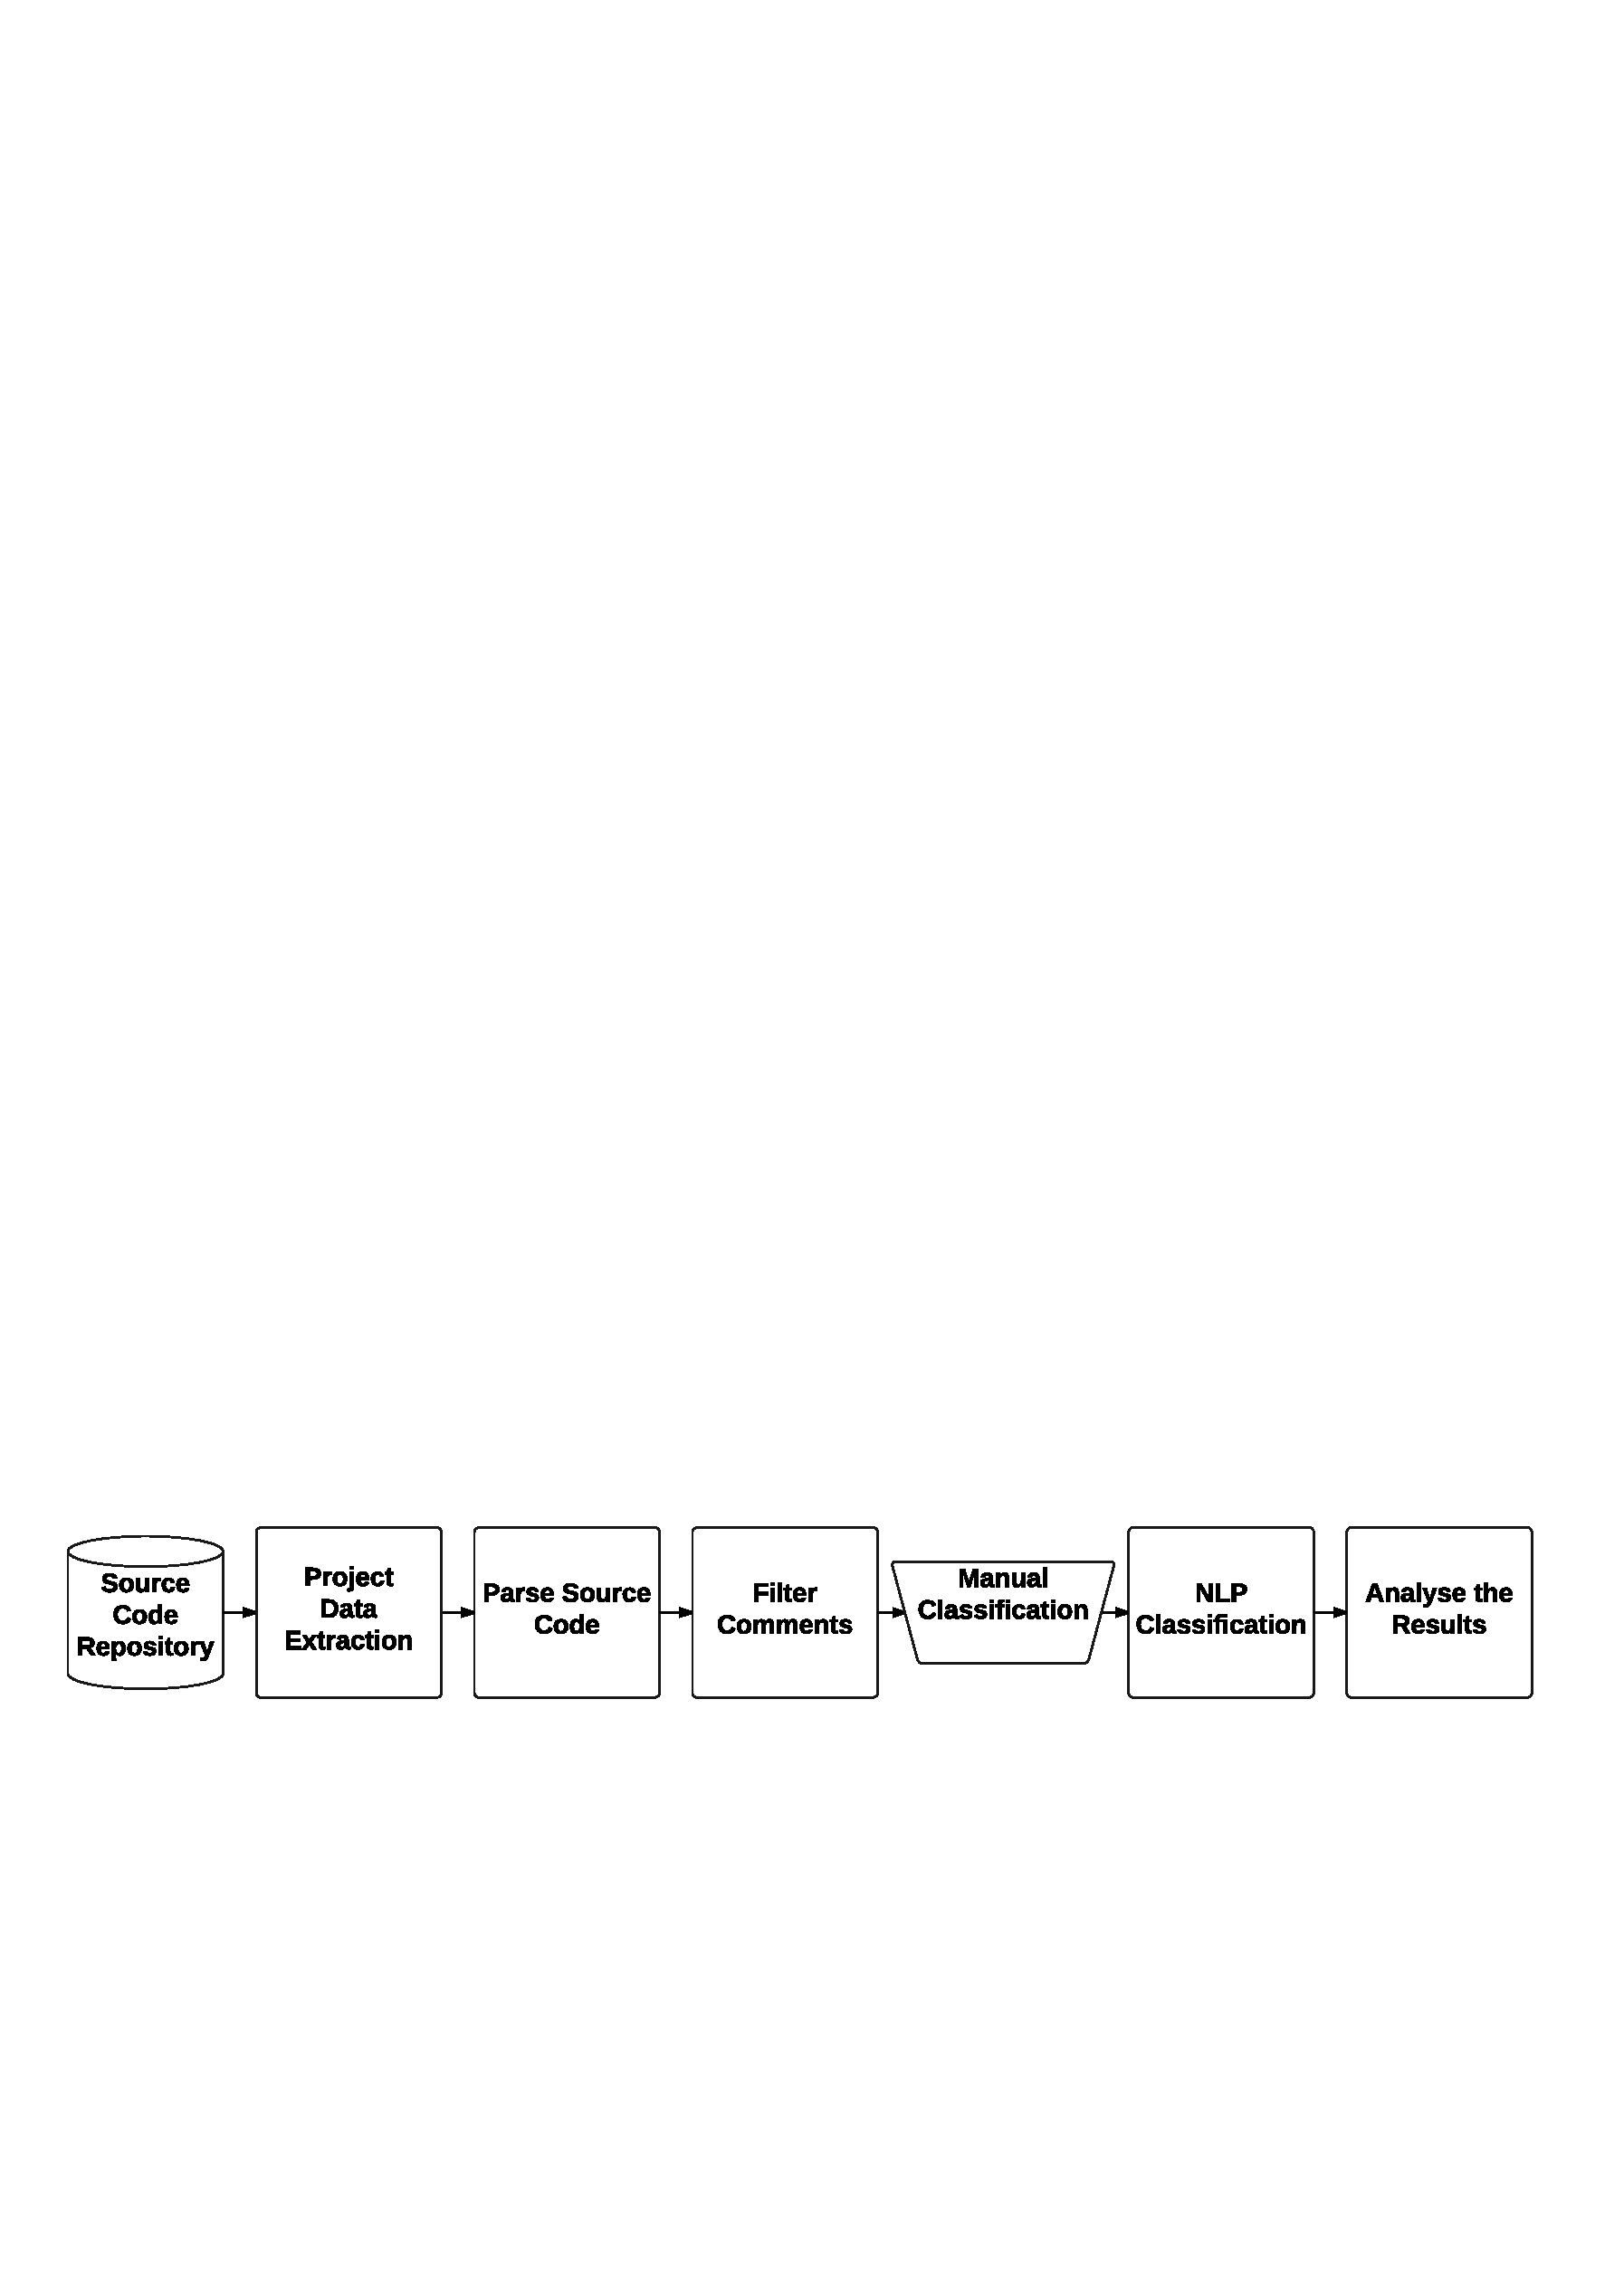
\includegraphics[width=1\textwidth]{figures/approach.pdf}
  \caption{Approach overview}
  \label{fig:approach}
\end{figure*}

The main goal of our study is to automatically identify \SATD trough source code comments. To do that, we first extract comments from ten open source projects. Second, we apply four filtering heuristics to remove comments that are irrelevant for the identification of \SATD  (e.g., license comments, commented source code and Javadoc comments). After that, we manually classify the remainder of comments into \SATD types (i.e., design debt, requirement debt, defect debt, documentation debt and test debt). Lastly, we use these comments as training data to the Stanford  Classifier. Figure~\ref{fig:approach} shows an overview of our approach, and the following subsections details each.

\subsection{Project Data Extraction} % (fold)
\label{sub:data_extraction}

To perform our study, we extract the source code of ten open source projects, namely Apache Ant, Apache Jmeter, ArgoUML, Columba, EMF, Hibernate, JEdit, JFreeChart, JRuby and SQuirrel. We selected these projects since they belong to different application domains, and vary in size (e.g., SLOC), and in the number of contributors. 

Table \ref{tab:project_details} provides more information about each one of the projects used in our study, listed in the first column. The second column provides the release used, followed by the number of classes, the total source lines of code (SLOC), the total extracted comments, the number of comments analyzed after applying our filtering heuristics, the number of comments that were classified as \SATD, the percentage of these comments that represent design debt, the percentage of \SATD comments classified as requirement debt and the number of contributors. 

A source line of code contains at least one valid character, which is not a blank space or a source code comment. In our study, we only use the Java files to calculate the SLOC, and to do so, we use the tool SLOCCount \cite{wheeler2004:home}. 

The number of contributors was extracted from OpenHub, an on-line community and public directory that offers analytics, search services and tools for open source software \cite{Openhub:home}. It is important to notice that the number of comments shown for each project does not represent the number of commented lines, but rather the number of individual line, block, and Javadoc comments. 

In total, we obtained 259,229 comments, found in 16,249 Java classes. The size of the selected projects varies between 81,307 and 228,191 SLOC's, and the number of contributors of these projects ranges from 9 to 326. 

\begin{table*}[!tbh]
    \begin{center}
    \caption{Project Details}
    \label{tab:project_details}
            \begin{tabular}{l| c c r c c c c c c c}
            \toprule
            \thead{Project}   & \thead{Release}  & \thead{\# of \\classes}   & \thead{SLOC} & \thead{\# of \\contributors}  & \thead{\# of \\comments}   & \thead{\# of \\comments \\after filtering} & \thead{\# of \\TD \\comments} & \thead{\% of \\Design \\Debt} & \thead{\% of \\Requirement \\Debt} & \thead{\% of \\Other \\Debts}\\ 
            \midrule 
            Ant            & 1.7.0    & 1,475 & 115,881 & 74  & 21,587 &  4,140  & 134   & 70.89 & 11.94 & 17.17\\
            ArgoUML        & 0.34     & 2,609 & 176,839 & 87  & 67,716 &  9,788  & 1,653 & 48.45 & 39.38 & 12.17\\
            Columba        & 1.4      & 1,711 & 100,200 & 9   & 33,895 &  6,569  & 295   & 42.71 & 45.42 & 11.87\\
            EMF            & 2.4.1    & 1,458 & 228,191 & 30  & 25,229 &  4,401  & 104   & 75.00 & 15.38 & 9.62 \\
            Hibernate      & 3.3.2 GA & 1,356 & 173,467 & 226 & 11,630 &  2,968  & 472   & 75.21 & 13.55 & 11.24\\
            JEdit          & 4.2      &   800 &  88,583 & 57  & 16,991 &  10,322 & 256   & 76.56 &  5.46 & 17.98\\
            JFreeChart     & 1.0.19   & 1,065 & 132,296 & 19  & 23,474 &  4,436  & 219   & 84.01 & 11.41 & 4.58 \\
            Jmeter         & 2.10     & 1,181 &  81,307 & 33  & 20,084 &  8,163  & 375   & 84.26 &  5.86 & 9.88 \\
            JRuby          & 1.4.0    & 1,486 & 150,060 & 328 & 11,149 &  4,901  & 626   & 54.79 & 18.21 & 27.00\\ 
            SQuirrel       & 3.0.3    & 3,108 & 215,234 & 46  & 27,474 &  7,330  & 386   & 54.14 & 38.86 & 7.00 \\ 
            \bottomrule             
        \end{tabular}
    \end{center}
\end{table*}


% subsection data_extraction (end)
\subsection{Parse Source Code} % (fold)
\label{sub:parse_source_code}

After obtaining the source code of all projects, we extract the comments from the source code. We use JDeodorant \cite{Tsantalis2008CSMR}, an open-source Eclipse plug-in, to parse the source code and extract the code comments. JDeodrant uses the Eclipse AST framework to create an Abstract Syntax Tree (AST) map of the source code. The AST map contains detailed information about the project such as: the source code comments, its type (i.e., Block, Single-line or Javadoc) and the line where each one of these comments begins and finishes. 

Due to these features, we adapted JDeodorant to extract the aforementioned information about source code comments and store it in a relational database to facilitate the processing of the data.

% subsection parse_source_code (end)
\subsection{Filter Comments} % (fold)
\label{sub:filter_comments}

Source code comments can be used for different purposes in a project like giving context, as part of the documentation, to express thoughts, opinions and authorship, and in some cases, to remove source code from the program. Comments are used freely for developers and with few formalities, if any at all. This informal environment allows developers to bring to light opinions, insights and even confessions (e.g., self-admitted technical debt). 

As shown in prior work by Potdar and Shihab \cite{Potdar2014ICSME}, part of these comments can be identified as self-admitted technical debt, but they are not the majority of cases. With that in mind, we develop and apply 4 filtering heuristics to narrow down the comments eliminating the ones that are less likely to be classified as self-admitted technical debt.

To do so, we developed a Java based tool that reads from the database the data obtained by parsing the source code. Next, it executes the filtering heuristics and stores the result back in the database. The retrieved data contains information like the line number that a class/comment begins/ends and the type, considering the Java syntax, of the comment (i.e., Block, Single-line or Javadoc). With this information we process the filtering heuristics as described next.

License comments are very not likely to contain self-admitted technical debt, and are commonly added before the declaration of the class. We create a heuristic that removes comments that are placed before the class declaration. Since we know the line number that the class was declared we can easily check for comments that are placed before that line and remove them. In order to decrease the chances of removing a self-admitted technical debt comment while executing this filter we calibrated this heuristic to not remove comments containing one of task-reserved words (i.e., ``todo'', ``fixme'', or ``xxx'').

Long comments that are created using multiples \emph{Single-line} comments instead of a \emph{Block} comment can hinder the understanding of the message considering the case that the reader (i.e., human or machine) analyzes each one of these comments independently. To solve that problem, we create a heuristic that searches for consecutive Single-line comments and groups them as one. We identify consecutive comments by subtracting the line number of both comments. If the result of the difference is equals a -1 we have a consecutive comment. For example, Single-line comment A is placed in line number 100 and Single-line comment B is placed in line 101. The subtraction of the line numbers will result in -1, therefore the comments are consecutive.
 
Commented source code is found in the projects due to many different reasons. One of the posible possibilities is that the code is not curently being used, other is that, the code is used for debuging purposes only. Based on our analysis, commented source code does not have self-admitted technical debt. Our heuristic remove commented source code using a simple regular expression that captures typical Java code structures.

Javadoc comments rarely mention self-admitted technical debt. For the Javadoc comments that does mention self-admitted technical debt, we notice that they usually contains one of the task-reserved words (i.e., ``todo'', ``fixme'', or ``xxx''). Therefore, our heuristic remove all comments of the type Javadoc unless they contain at least one of the task-reserved words. To do so, we create a simple regular expression that search for the task-reserved words before removing the comment.  

The steps mentioned above significantly reduced the number of comments in our dataset and helped us focus on the most applicable and insightful comments. For example, in the Apache Ant project, applying the above steps helped reduce the number of comments from 21,587 to 4,140 comments meaning that 19.17\% of the comments were kept for analysis. The percentage of comments that were kept for analysis ranges from 14.45\% to 40.64\%. Table \ref{tab:project_details} provides the number of comments kept after the filtering heuristics for each project.
% subsection filtering_comments (end)

\subsection{Manual Classification} % (fold)
\label{sub:manual_classification}

To classify the comments, we developed a Java based tool that shows one comment at a time and gives a list of possible classifications that can be manually assigned to the comment. The list of possible classifications is based on previous work ~\cite{Alves2014MTD}. After applying the different filtering steps, we successfully classified more than 63 thousand comments into five different types of self-admitted technical debt: design debt, defect debt, documentation debt, requirement debt and test debt.

 In total we read and classified 63,015 comments from ten open source projects. The classification took approximately 185 hours and was performed by the first author of the paper.  

To mitigate the risk of creating a dataset too biased we created a significative sample of our dataset and asked for a master student to classify it. To prepare the student for this task we gave an 1 hour explanation about the different kinds of \SATD, and walked the student throught a couple of examples of each diferent type of \SATD comment. 

The signicative sample was created based on the total number of comments (63,015) with a confidence level of 99\% and a confidence interval of 5\%. Wich means that the significative sample has 659 comments. We composed significative sample accordingly with the percentage of each classification found in the original dataset. Therefore, the significative sample was comporsed of: 92\% of comments with no \SATD (609 comments), 4\% of design debt comments (29 comments), 2\% of requeriments debt comments (5 comments), 0.75\% test debt (2 comments) and 0.15\% of documentation debt (1 comment).

Lastly, we evaluate the level of agreement between both reviewers of the significative sample by calculatint the Cohen's kappa coefficient ~\cite{cohen1960coefficient}. The level of agreement measured between the reviewers was of \todo{}.   
 
% subsection manual_classification (end)

% subsection heuristics_to_remove_irrelevant_comments (end)
\subsection{Run the NLP Classifier} % (fold)
\label{sub:run_the_nlp_classifier}

\todo{explain in detail the npl tool , why we use it and how it works.} 

Our next step is to use the classified \SATD comments to create a training dataset that can be used with a NLP classifier. A NPL classifier is a machine learning tool that take as input a number of data items along with the classification that this data item belongs, we choose to use the Stanford Classifier ~\cite{Manning2014ACL} as our machine learning tool. In our case, the training data is composed by a comment and the manual classification that was attributed to it. According to our findings in previous work \cite{Maldonado2015MTD} the most frequent types of \SATD are design debt, implementation debt and defect debt, and therefore we focuses our approach in the prediction of these two types of \SATD comments.

For each comment in our training dataset we remove the characters structures and symbols that are inherent from the Java language syntax and used to indicate a comment (i.e., `//' or `/* and */') or that represent a escape sequence such as `\textbackslash t' or `\textbackslash n'. We also remove the excess of blank spaces from the comments, and the resulting sentence is added to training dataset with its classification. Lastly, we make all the comments lowercase, to create a more uniform training dataset.  

After creating the training dataset we also create a test dataset in order to measure to performance of the Stanford Classifier in predicting \SATD comments. The test dataset is created following the same formatting rules as described above for the training dataset. 

% subsection run_the_nlp_classifier)
